\documentclass[11pt]{article}
\usepackage[letterpaper,margin=1in]{geometry}
\usepackage[T1]{fontenc}
\usepackage[utf8]{inputenc}
\usepackage{lmodern}
\usepackage{microtype}
\usepackage{graphicx}
\usepackage{booktabs,tabularx,longtable,array}
\usepackage{xcolor}
\usepackage{caption}
\usepackage{enumitem}
\usepackage{amsmath}
\usepackage{url}
\usepackage{newunicodechar}
\usepackage[colorlinks=true,linkcolor=blue!50!black,citecolor=blue!50!black,urlcolor=blue!50!black]{hyperref}
\usepackage{xurl}
\newunicodechar{≤}{\ensuremath{\leq}}
\newunicodechar{≥}{\ensuremath{\geq}}
\newunicodechar{≈}{\ensuremath{\approx}}
\newunicodechar{−}{\ensuremath{-}}
\setlength{\parskip}{4pt}\setlength{\parindent}{0pt}
\emergencystretch=2em
\title{An AI Agent Team in a Robot-Learning Challenge: A Case Study}
\author{Ahmet Ercan Batirel\\Imitation.Tech\\\texttt{aebatirel@gmail.com}}
\date{November 2026}
\begin{document}
\maketitle
\begin{abstract}
Can a team of AI coding agents, directed by one person, take a robot-learning problem from raw human video to a ranked competition entry? We report one case. In the NVIDIA V2D Challenge, Track 3 (Kaggle, October–November 2026), a human owner directed about 20 Claude Code cloud sessions. The sessions built the whole pipeline: stereo depth, detection and 6D tracking of objects in egocentric video, object meshes, robot-hand references and grasps, reinforcement-learning (RL) policies for a simulated hand pair trained on rented GPUs, and the packing and upload of submissions. They worked under written rules on integrity and spending.

Over 26 uploads the main score (AUC) rose from 0.575 to 0.886. The rank sum over six boards placed the team 7th on 3 November and 8th on 6 November. The main technical finding is that the remaining error came from bias in the reconstructed object poses, mostly while objects were held, not from policy following: at the end every policy passed the success thresholds against our own references. The main process findings are that pre-registered pass marks held under pressure (about 96 failed or declined tests were logged with their margins), that the largest gains came from fixing gross failures and from reading the scorer's code, and that the human principal stepped in often. GPU rental cost about \$556 {[}E{]}. AI usage would have cost about \$7,100 at API list prices across 20 sessions; in practice it ran on a \$200 Claude Code subscription plus \$250 of cloud credit gifted by Anthropic, so the binding limit was the usage cap, not money.

\end{abstract}
\section{Introduction}
People handle objects with skill in everyday video. Turning such video into robot policies is an old goal \cite{r1,r2} and an active one \cite{r3,r4,r5,r6}. The usual route has three steps. First, reconstruct the objects and their motion from the video. Second, turn the human motion into a reference that a robot hand can follow. Third, train a policy, usually in simulation, to make the objects move as they did in the video.

The V2D Challenge, Track 3 \cite{r7}, tests this route on hidden data. Teams receive head-mounted stereo videos of a person handling kitchen objects. They submit object meshes and simulated robot rollouts. The scorer compares the simulated object motion with motion capture that teams never see.

We entered with an unusual team. One human, the owner, set goals, approved spending and ruled on integrity questions. The engineering and research were done by about 20 cloud sessions of Claude Code, Anthropic's coding agent \cite{r8}. Agent systems that run research are now common in the literature \cite{r9,r10}, including in robot learning \cite{r11,r12}. So are concerns about their integrity \cite{r13,r14}. Most published accounts score themselves or use fixed tasks. Ours was scored by a live competition on hidden episodes, against human teams, with real money spent on rented GPUs.

This is a case study: one project, with no control group. Its value is in the detail. We report what was tried, what it cost, what failed and by how much, and where the human had to step in. The full record exists: git history, work logs, pre-registrations and session transcripts. Every number here comes from it.

Our contributions are:

\begin{enumerate}[itemsep=2pt,topsep=3pt]
\item \textbf{A technical error decomposition.} We trace the score from 0.575 to 0.886 AUC to specific levers, and show that the remaining error was bias in the reconstructed poses, not policy following.
\item \textbf{A catalogue of pre-registered negative results.} About 96 failed or declined tests, each with its pass mark and margin. About 20 ground-truth-free perception ideas all missed their gates.
\item \textbf{A scorer analysis.} The scorer registers the submitted mesh to a hidden scan and aligns the scene once at frame 0, so the mesh is a first-order term of every pose score. We found this late; mesh changes were then worth about 0.04 AUC with no retraining.
\item \textbf{An end-to-end account of an agent team under governance.} We describe its roles, rules, error types, owner interventions and costs, backed by a full audit trail.
\end{enumerate}
Section 2 reviews related work. Sections 3 to 5 describe the challenge, the team and the pipeline. Sections 6 to 8 give the results, the failures and the process analysis. Sections 9 and 10 give lessons and limitations.

\section{Related work}
\subsection{Learning robot manipulation from human video}
DexMV \cite{r1} built an early pipeline from human video to dexterous robot imitation: estimate hand and object poses, retarget the hand to a robot, and learn from the result. Patel et al. \cite{r2} reconstructed object interactions from internet videos and trained simulated policies to imitate them. Later work puts the object, not the hand, at the centre and adds physics. ManipTrans \cite{r3} transfers bimanual human manipulation to robot hands with residual learning. DexTrack \cite{r4} learns a general tracking controller for human hand–object references. Dexplore \cite{r15} learns control through exploration scoped around the references. DexMachina \cite{r5} uses virtual object controllers whose strength decays during training. The kit we used has the same kind of fading assist. SPIDER \cite{r6} uses physics-informed retargeting to make human motion feasible for a robot.

Work from 2026 starts from egocentric video. EgoAERO \cite{r16} learns dexterous manipulation from a single egocentric video without object assets. EgoEngine \cite{r17} turns egocentric human videos into robot demonstrations. Grasp-and-Lift \cite{r18} reconstructs hand–object interaction with physics in the loop, and CRISP \cite{r19} uses contact guidance to build simulation scenes from monocular video. Eureka \cite{r20} showed that language models can write reward functions for dexterous RL.

Our pipeline follows this line closely. Its object-centred reference, its fading assist and its per-episode RL are not new. What differs is the setting: hidden ground truth, a fixed robot and simulator, and a scorer we had to learn from its code.

\subsection{Object and hand–object reconstruction}
Our perception stack was assembled from published models. FoundationStereo \cite{r21} gives zero-shot depth from a stereo pair. FoundationPose \cite{r22} registers and tracks a novel object given its mesh. SAM 2 \cite{r23} segments images and video. OWLv2 \cite{r24} detects objects from text prompts, and DINOv2 \cite{r25} gives general image features. Our detector follows CNOS \cite{r26}, which matches segment proposals against renders of a mesh, and we tested the scores of SAM-6D \cite{r27}. MediaPipe Hands \cite{r28} gives 2-D hand landmarks. Meshes came from volumetric depth fusion \cite{r29}.

Joint shape-and-pose methods such as BundleSDF \cite{r30} and Any6D \cite{r31}, and hand–object methods such as HOLD \cite{r32}, MagicHOI \cite{r33} and HaWoR \cite{r34}, were reviewed but not run. The hand–object methods are monocular and take hours per sequence, and joint shape and pose was judged to be days of work. For one test we adopted the object term of HOnnotate's objective \cite{r35}. Simulation used MuJoCo \cite{r36} in its GPU form, MuJoCo Warp \cite{r37}, with convex collision pieces from CoACD \cite{r38}.

\subsection{AI agents running research}
The AI Scientist \cite{r9} and its successors \cite{r39,r40} automate the loop from idea to paper in computational machine learning. Agent Laboratory \cite{r10} uses agents as research assistants, with human feedback between stages. The AI co-scientist \cite{r41} generates and debates hypotheses with several agents. Coscientist \cite{r42} planned and ran chemistry experiments. Shen et al. \cite{r43} study how several agents collaborate in automated research. Trehan and Chopra \cite{r44} report four autonomous research attempts and why they fell short. Benchmarks measure parts of the job: MLE-bench \cite{r45} uses offline Kaggle competitions, RE-Bench \cite{r46} compares agents with human experts on research engineering, and PaperBench \cite{r47} asks agents to replicate papers.

Robotics is closer to our case. ENPIRE \cite{r11} uses agents to improve robot policies in the real world; by its authors' account, several coding agents coordinate through git. Khandelwal and Gupta \cite{r12} report an agent that ran more than 70 RL experiments on quadruped locomotion while a human set the direction. Lei et al. \cite{r48} use digital agents as coaches for embodied policies and test them on 32 RL and imitation-learning tasks. These are the closest precedents. Agents running RL loops, and several agents coordinating through git, are not new. But these works start from a given robot task and environment, not from human video, and none was judged by an external competition. In our search, which was not exhaustive, we found no report of an agent-built entry in an embodied-AI competition.

\subsection{Integrity of agent-run research}
Research agents can game their own metrics. Huang et al. \cite{r13} show reward hacking by autonomous research agents. Atinafu and Cohen \cite{r49} benchmark evaluation integrity for ML-engineering agents, including locking the evaluator. A recent survey \cite{r14} names the gap between what agents claim and what is verified. Pre-registration is the classic remedy in science \cite{r50}. Vaccaro \cite{r51} argues for it in experiments with AI agents, and K-Dense \cite{r52} commits predictions to git before results arrive. Our practice of committing pass marks to git before scoring has these close precedents. What we add is a record of it in use: many tests, real money, a hidden test set, and the near-misses it rejected.

\section{The challenge}
From here on we mark numbers as \textbf{{[}M{]}} measured (on the leaderboard, in the billing record, or on public episodes against mocap), \textbf{{[}E{]}} estimate, \textbf{{[}H{]}} hypothesis and \textbf{{[}I{]}} inference. Public-episode measurements use ground truth for scoring only, never for inference. Board numbers without a label are {[}M{]} from the Kaggle record.

\subsection{Task and data}
Each episode is a short head-mounted stereo video of one person handling one or two kitchen objects: pots, cups, a lid, a pitcher, a dish rack, a sweeper, a dust pan, two wooden boards and a wooden spoon. A team must (1) reconstruct each object's mesh, (2) estimate each object's 6-DoF trajectory, and (3) train a simulated pair of robot hands so that the simulated objects follow that trajectory \cite{r7}. The robot is the kit's five-finger Sharpa hand pair in MuJoCo Warp. Kaggle scores the simulated object motion against hidden motion capture (mocap), and the meshes against hidden scans.

There are 20 public episodes with mocap and scans, for development, and 20 eval episodes without them, for the leaderboard. The public set has 5,246 frames at 20.25 frames per second; 13 of its 20 episodes have two objects. Public mocap holds object poses only: no hands and no camera. The wooden spoon is in 10 of the 20 eval episodes and anchors the scene in five, but it has no public scan or mocap. Uploads closed on 4 November 2026.

\subsection{Six boards and a rank sum}
\begin{table}[tbp]
\centering\small
\begin{tabularx}{\linewidth}{l>{\raggedright\arraybackslash}Xl}
\toprule
\textbf{Board} & \textbf{What it measures} & \textbf{Better} \\
\midrule
AUC & per frame and object, the position error mapped to a score (1 below 1 cm, 0 at 9 cm), averaged over the 20 episodes & higher \\
SP-SR & share of episodes with mean position error ≤ 10 cm and mean orientation error ≤ 0.5 rad & higher \\
MP-SR & share of episodes in which every object stays under 3 cm and 30 degrees & higher \\
RPE (cm) & error of the second object's position in the first object's frame & lower \\
MPPE (cm) & mean position error per object & lower \\
CD-O (cm) & Chamfer distance between our mesh and the hidden scan, after a similarity fit & lower \\
\bottomrule
\end{tabularx}
\end{table}
One episode is worth 0.05 on each success board. The final rank is the sum of a team's six board ranks, and each board keeps the team's best upload. So an upload that is worse on five boards and better on one costs nothing. We assumed that AUC alone decided the rank until 31 October.

\subsection{How the scorer treats a submission}
Two facts about the scorer shaped the project. We learned both from its code; the second we understood fully only on 2 November.

\begin{itemize}[itemsep=2pt,topsep=3pt]
\item \textbf{Frame-0 alignment.} The scorer aligns the whole simulated scene once, at frame 0. Rotation comes from the first object without a symmetry axis, translation from the object in slot 0. Any error in that anchor reaches every object and every frame.
\item \textbf{Mesh registration.} The scorer registers our submitted mesh to the hidden scan with trimmed ICP \cite{r53,r54} from 25 starts, and converts our poses through that fit. So the submitted mesh changes the pose boards, not only CD-O. On six public episodes, a clean scan scored 0.987 AUC; the same scan with 3 mm of noise scored 0.825, and with 5 mm of inflation 0.608 {[}M{]}.
\end{itemize}
Nothing is re-run on Kaggle: the submitted rollouts are scored as they are. Results stay provisional until the organisers reproduce each counted file in their own container.

\subsection{Our integrity rules}
The owner set the working rules in the repository's instruction file, which every session read first. On 20 October he reviewed 29 proposed rules and removed or changed about a third. The rules that matter here:

\begin{itemize}[itemsep=2pt,topsep=3pt]
\item \textbf{No ground truth in inference.} Mocap, scans and the pose fields of the public episode files were read only for scoring and diagnosis. Object names and slot order were allowed, because the kit gives them for eval episodes too. From 30 October a leak guard in the packing scripts refused inputs that had touched ground truth.
\item \textbf{GT-informed choices disclosed and owner-approved.} From 2 November some submitted meshes were chosen among ground-truth-free candidates by their Chamfer distance to public scans. The owner approved each step, and every upload description says so. Other disclosed items: one policy trained with a larger contact buffer than the evaluator uses, one waived clause of the swap rule, and one revert informed by a board result (pack 6).
\item \textbf{No tuning on leaderboard results.} Public development and eval inference were kept apart. Thresholds set after seeing scores, and ``best per board'' variants, were refused as probes of the hidden set.
\item \textbf{Spending.} State the plan and the expected cost before each rental batch. Every machine destroys itself when its job ends, and a watchdog destroys a machine that has stalled for about 30 minutes.
\end{itemize}
\section{How the agent team worked}
\subsection{Roles}
\begin{itemize}[itemsep=2pt,topsep=3pt]
\item \textbf{The owner} was the principal. He set the goals (``aim for 4th place'' on 25 October, ``reach top 3'' on 2 November), approved spending, uploads and every exception to the rules, and kept registration and contact with the organisers to himself. He made 8 of the 2,359 commits.
\item \textbf{Advisors.} An external advisor met the team twice (30 and 31 October, about 30 minutes each), and a professor gave feedback on 31 October. The advisor asked about hands, masses, and bias versus noise. The professor pointed at rollout variance and at the split between reconstruction and control.
\item \textbf{The main early session} (20–27 October) set up the rented GPUs, built the first stack and produced the first packs.
\item \textbf{The builder session} (26 October – 3 November) built packs and ran carry, contact and error-decomposition studies.
\item \textbf{The coordinator session} (30 October – 6 November) analysed advisor input, relayed work between sessions, and from 1 November was the single uploader to Kaggle.
\item \textbf{Fourteen lane sessions} each ran one workstream: mesh generation, perfect following, embodiment, policy review, comparison with NVIDIA's method, score status, perception accuracy, a grasp sampler, team registration, physics priors, a room map, point tracks, a pot pose network and hand-aware tracking. Three short sessions did reviews and side questions.
\end{itemize}
Until 25 October the work ran mostly in one session. A few parallel sessions were added on 25–26 October, and the coordinated lane team started on 30–31 October.

\begin{figure}[tbp]
\centering
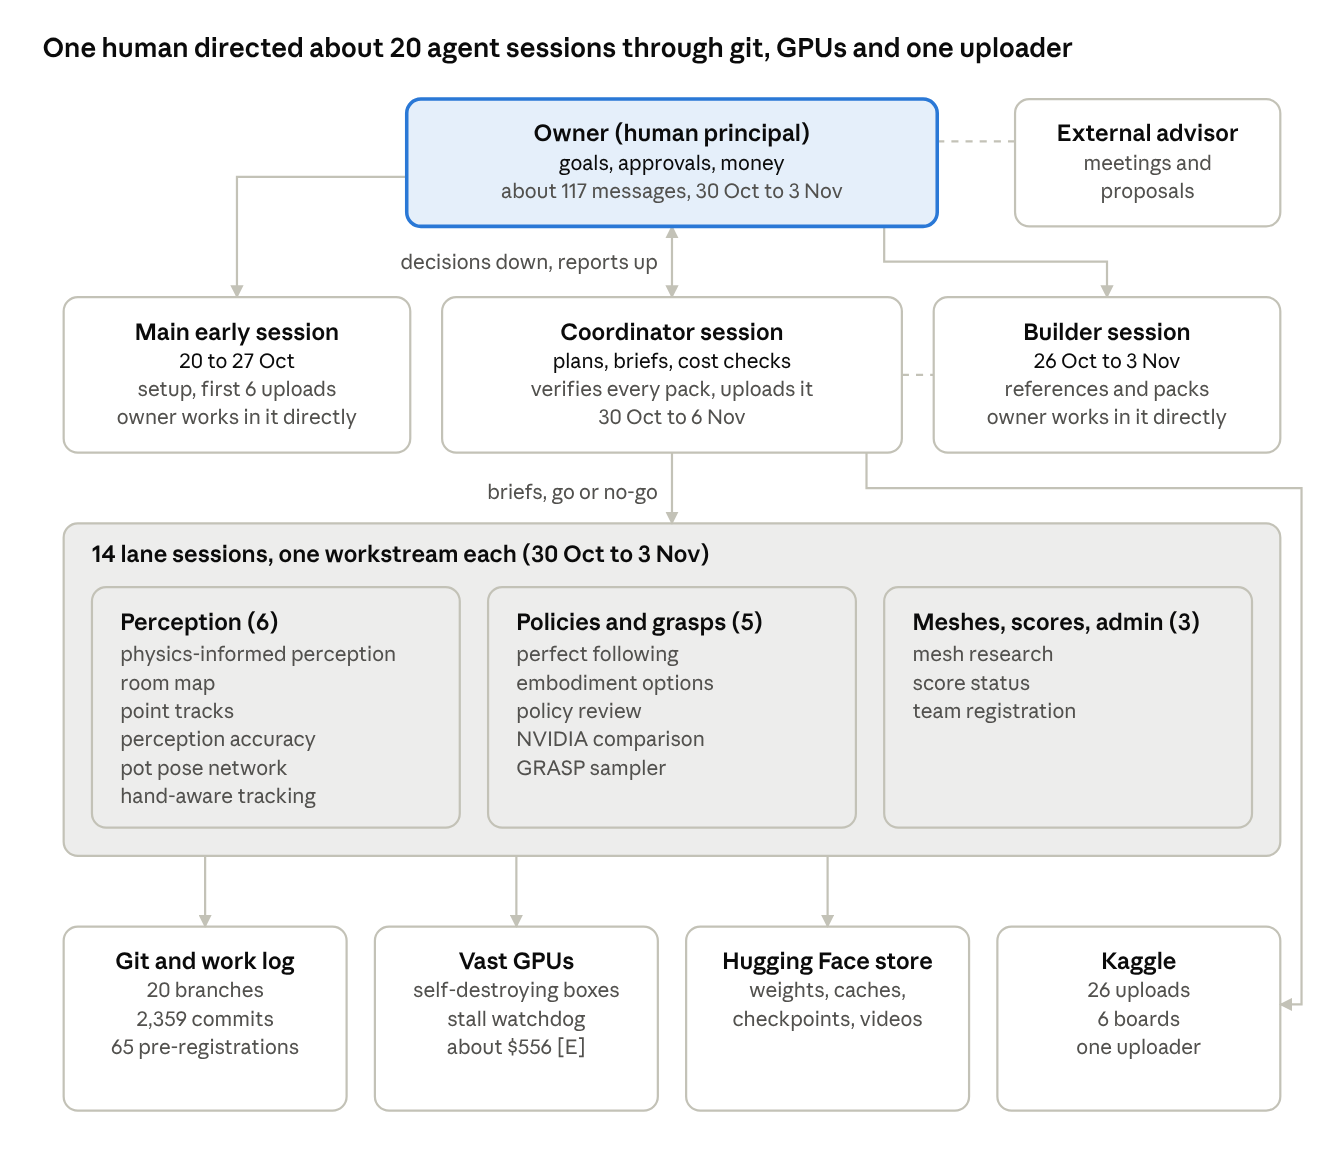
\includegraphics[width=0.92\linewidth]{figures/fig01_team.png}
\caption{The team. The owner directs the coordinator session, which relays work to the lane sessions; every session writes to git branches and the shared work log; rented Vast GPUs run the jobs and write to a private store; one session uploads to Kaggle. The human holds direction, money and exceptions; the agents hold the engineering.}
\label{fig:1}
\end{figure}
\subsection{Communication}
The sessions did not share memory or context. They shared four things:

\begin{enumerate}[itemsep=2pt,topsep=3pt]
\item \textbf{Git.} Twenty branches in all; on 30 October one lane merged every existing branch into \texttt{main}. Each session committed code, results, pre-registrations and small checkpoints.
\item \textbf{A status file and a work log.} Every session started by reading the status file and the rules, and appended a dated entry to the work log after each result: 362 unique entries in all.
\item \textbf{Cross-session messages,} sent by the coordinator or relayed by the owner.
\item \textbf{A shared spend ledger} in the private store, with a ``planned'' line before each machine and an ``actual'' line after it. It came in on 29 October, when three sessions drew on one budget.
\end{enumerate}
GPU machines were rented through the Vast API \cite{r55}. The agents' sandbox could not open SSH connections for the whole project. So machines were watched through Vast labels, the Vast log API, uploads to the store every 30 minutes and an HTTPS terminal.

\subsection{Governance}
\begin{table}[tbp]
\centering\small
\begin{tabularx}{\linewidth}{l>{\raggedright\arraybackslash}X>{\raggedright\arraybackslash}X}
\toprule
\textbf{Mechanism} & \textbf{What it required} & \textbf{Why and when} \\
\midrule
Pre-registration & pass mark, falsifier and analysis committed to git before results (65 files) & to stop rules being chosen after scores are seen (24 Oct) \\
No best-of-N draws & a packed rollout must be a fresh run of the chosen checkpoint & the owner's ``we cannot pick and choose'' (25 Oct); packed draws later proved lucky \\
Single-twin ban & a mesh swap needs two public twins or a reference-free argument & the lathe pitcher failure (26 Oct) \\
Swap rule & 10 fresh runs, a gain of at least +0.02, no more failed runs, median RPE not worse & pack 9b (1 Nov) \\
Two-host confirmation & a swap must also pass on fresh runs on a second machine & drops of 0.10–0.17 from training box to fresh runs (3 Nov) \\
Plan and cost first & plan, expected cost and a credit floor stated before each rental batch & the repository rules (20 Oct) \\
Self-destroying machines & each machine destroys itself; a watchdog kills one stalled for about 30 minutes & the repository rules (20 Oct) \\
Leak guard and one uploader & packing refuses GT-touched inputs; one session uploads, with checksums & a packing bug (26 Oct) and a crossed upload (31 Oct) \\
\bottomrule
\end{tabularx}
\end{table}
A safety check in the agent product also acted as governance. Between 31 October and 2 November it refused six owner approvals relayed from another session, and it blocked several upload commands. Each time the agent reported it and waited for the owner's own words. On the evening of 2 November the owner wrote: ``Upload 13b, you dont need my permission to upload anymore.''

\subsection{Phases}
\begin{table}[tbp]
\centering\small
\begin{tabularx}{\linewidth}{ll>{\raggedright\arraybackslash}Xl}
\toprule
\textbf{Phase} & \textbf{Dates} & \textbf{Main work} & \textbf{Best AUC at end} \\
\midrule
0 Side research & 1–12 Oct & baseline review, error budget on public mocap, perception survey & – \\
1 Building the stack & 12–23 Oct & perception, rented GPUs, first end-to-end runs, grasp lock, spoon recipe & – \\
2 First uploads & 24–26 Oct & packs 1–6; reference rebuild and learner choice & 0.81391 \\
3 Small swaps & 27–30 Oct & robustness review, mesh research, pack 7 & 0.81460 \\
4 Rank sum and eval 10 & 31 Oct – 1 Nov & CD-O found at 18th; lanes start; contact-buffer fix & 0.83921 \\
5 Meshes as a pose lever & 2 Nov & 12 uploads; the scorer's code read & 0.88571 \\
6 CD-O variants & 3 Nov & three mesh-only uploads; lanes closed & 0.88571 \\
\bottomrule
\end{tabularx}
\end{table}
\subsection{Where the human stepped in}
The owner's interventions were of five kinds:

\begin{itemize}[itemsep=2pt,topsep=3pt]
\item \textbf{Direction.} ``fix the lower scores properly, do whatever it takes, aim for 4th place'' (25 October); ``get me into that top tier'' (31 October).
\item \textbf{Rulings.} Own meshes only on eval episodes (21 October); per episode, use whichever of two learners follows better (``use both'', 25 October); no cherry-picked runs (25 October); approval of the GT-informed mesh selection (2 November).
\item \textbf{Money.} Each credit top-up; no budget cap for the work (30 October); a \$6 cap for one machine that overrode the no-time-limit rule.
\item \textbf{Corrections.} He asked for a cheap physics replay before a 55 GPU-hour plan (26 October). He queried a cost estimate, which then fell from \$400–900 to \$40–70 (3 November). He corrected an agent's label of a video shown to the advisor (31 October).
\item \textbf{Waivers.} One clause of the swap rule, for eval 15 (2 November).
\end{itemize}
He sent about 117 messages to the coordinator in its first five days (section 8).

\section{The technical pipeline}
\begin{figure}[tbp]
\centering
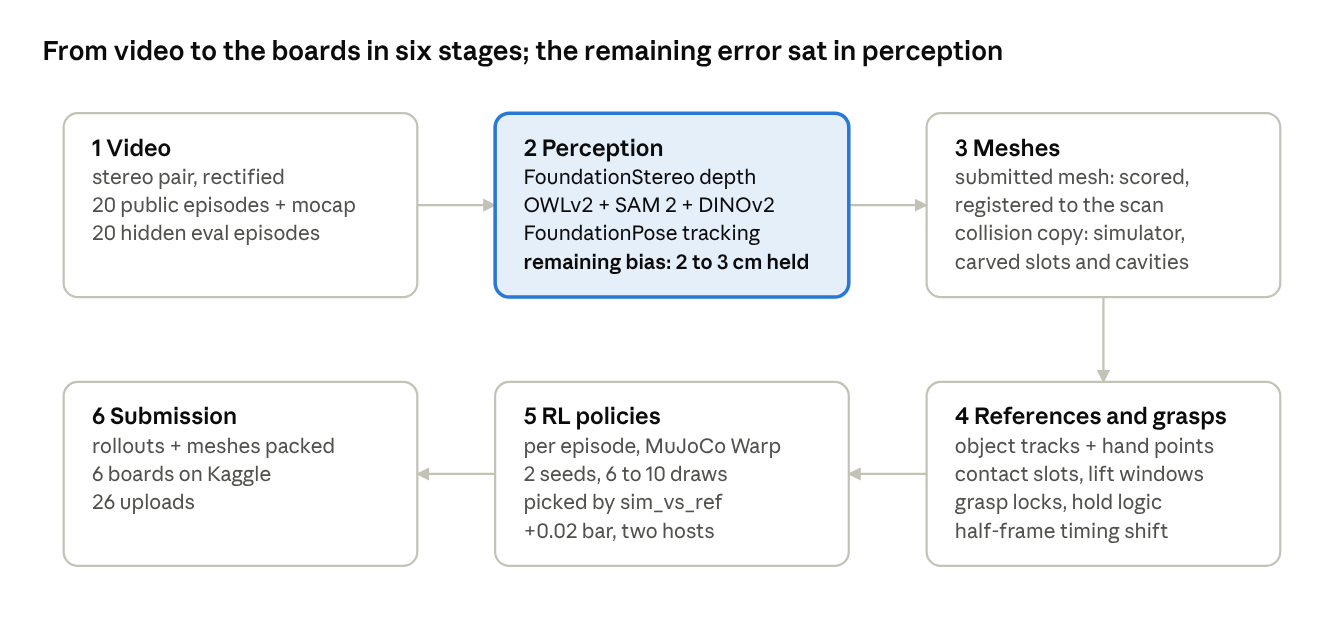
\includegraphics[width=\linewidth]{figures/fig02_pipeline.png}
\caption{The pipeline. Stereo video goes through depth, detection and 6D tracking; meshes are built from our own depth or generated; references and grasps are made from the object tracks and hand landmarks; RL policies are trained per episode in simulation; rollouts and meshes are packed and uploaded. Each stage was owned by one or more sessions.}
\label{fig:2}
\end{figure}
\subsection{Perception}
\begin{table}[tbp]
\centering\small
\begin{tabularx}{\linewidth}{>{\raggedright\arraybackslash}X>{\raggedright\arraybackslash}X>{\raggedright\arraybackslash}X}
\toprule
\textbf{Component} & \textbf{Role} & \textbf{Evidence {[}M{]}} \\
\midrule
FoundationStereo \cite{r21}, half resolution & metric depth from the 7.5 cm stereo pair & public ep12: AUC 0.997, MPPE 0.52 cm \\
Detector after CNOS \cite{r26}: SAM 2 \cite{r23} proposals scored by DINOv2 \cite{r25} features against 42 renders of each mesh, with a 3-D size gate and Hungarian assignment & find each listed object at frame 0 & replaced OWLv2 \cite{r24}, which missed the pot on grey frames and swapped two twin cups \\
FoundationPose \cite{r22} & register and track each object's 6-DoF pose & median position error 0.3–2.3 cm when detection is right \\
Detection rules (a 1,248-variant grid, then a gated re-proposal and an on-table rule) & reject people, chairs and object parts & correct public instances 78 → 97 of 116, none lost \\
Track guard & flag tracks that sink more than 2 cm under the table, then retry & fires on exactly the 3 known public failures \\
Board identity rule & name the two look-alike boards by knob darkness & public ep24: 0.029 → 0.706 \\
MediaPipe Hands \cite{r28} on the colour camera & 2-D hand landmarks & two hands in 173 of 181 frames (ep12) \\
\bottomrule
\end{tabularx}
\end{table}
On public episodes the tracking AUC rose from 0.809 (13 October) to 0.932 (20 October). Under the full scorer with our own meshes it reached 0.945 on 19 episodes by 2 November {[}M{]}.

On eval episodes the reference was much worse. Pack 1's rollouts followed our own references at 0.710, but the board gave 0.575. So about 0.135 AUC was reference-versus-truth error, against 3–4 \% on the public twins {[}M{]}. One cause was the wearer's white smartwatch: cups and the sweeper latched onto the wrist in four eval episodes.

\begin{figure}[tbp]
\centering
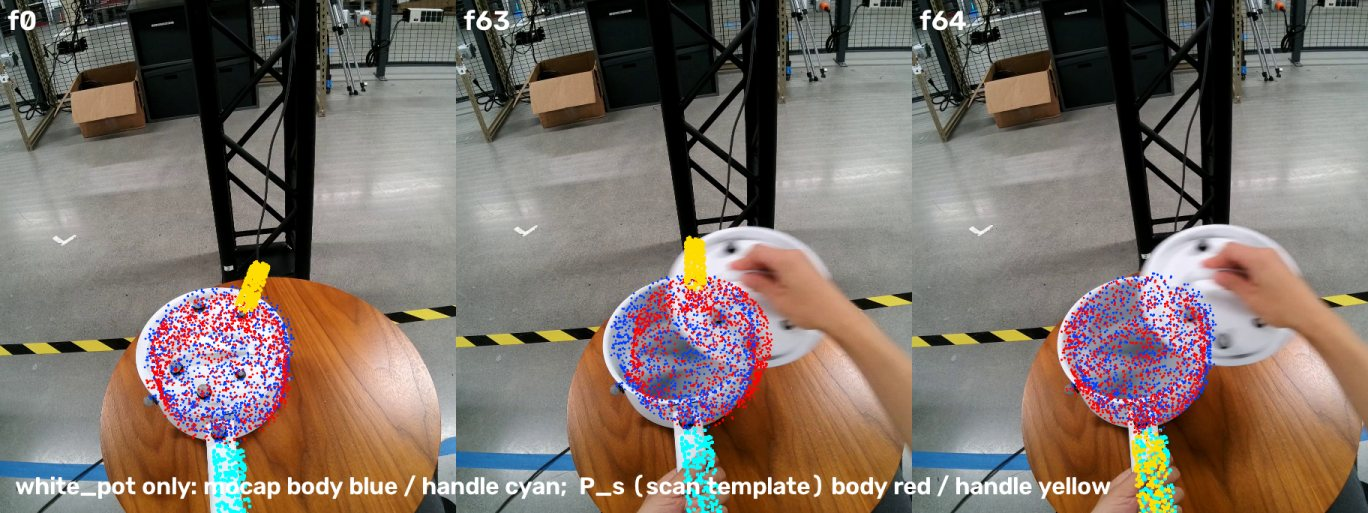
\includegraphics[width=\linewidth]{figures/fig03_tracking_flip.jpg}
\caption{A gross perception failure on public episode 0: the pot's 6D track flips between frames 63 and 64. The mocap overlay is drawn for diagnosis only; inference never saw it.}
\label{fig:3}
\end{figure}
\subsection{Meshes: what we submit and what the simulator touches}
A mesh did three jobs, and the best mesh for one job was often not the best for another. It was a tracking template for FoundationPose, the submitted mesh that Kaggle scores and registers, and a collision copy that only the simulator sees.

\begin{itemize}[itemsep=2pt,topsep=3pt]
\item \textbf{Submitted meshes.} We built them from our own depth along our own tracks by volumetric fusion \cite{r29}, with fixes for undersides the camera never sees (the pot first came out 5.5 cm below the table). Round objects were rebuilt by revolving their observed profile, and the pot, lid and rack from primitive parts. Late in October we added candidates from image-to-3D generators. From 2 November we chose among candidates by their Chamfer distance to public scans (GT-informed, disclosed).
\item \textbf{Collision copies.} CoACD \cite{r38} splits a mesh into convex pieces, but it inflates surfaces by 2.9–12.6 mm and refills slots and cavities. Pack 4 carved the eval-10 cup cavity and the eval-25 board slots in the collision copies only, leaving the submitted meshes unchanged. With two small rollout fixes, it gave +0.02163 AUC.
\item \textbf{Meshes as a pose lever.} The scorer registers the submitted mesh, so the mesh with the best Chamfer distance is not always the best to submit. Pack 13i swapped in a pot with a better Chamfer distance but 6.8 mm of registration error, against 2.7 mm for the pot it replaced. With two other mesh changes, AUC fell by 0.004. From 2 November, pose-board meshes were chosen by public leave-one-episode-out cross-validation with 10 registration seeds, excluding each mesh's source episode.
\begin{figure}[tbp]
\centering
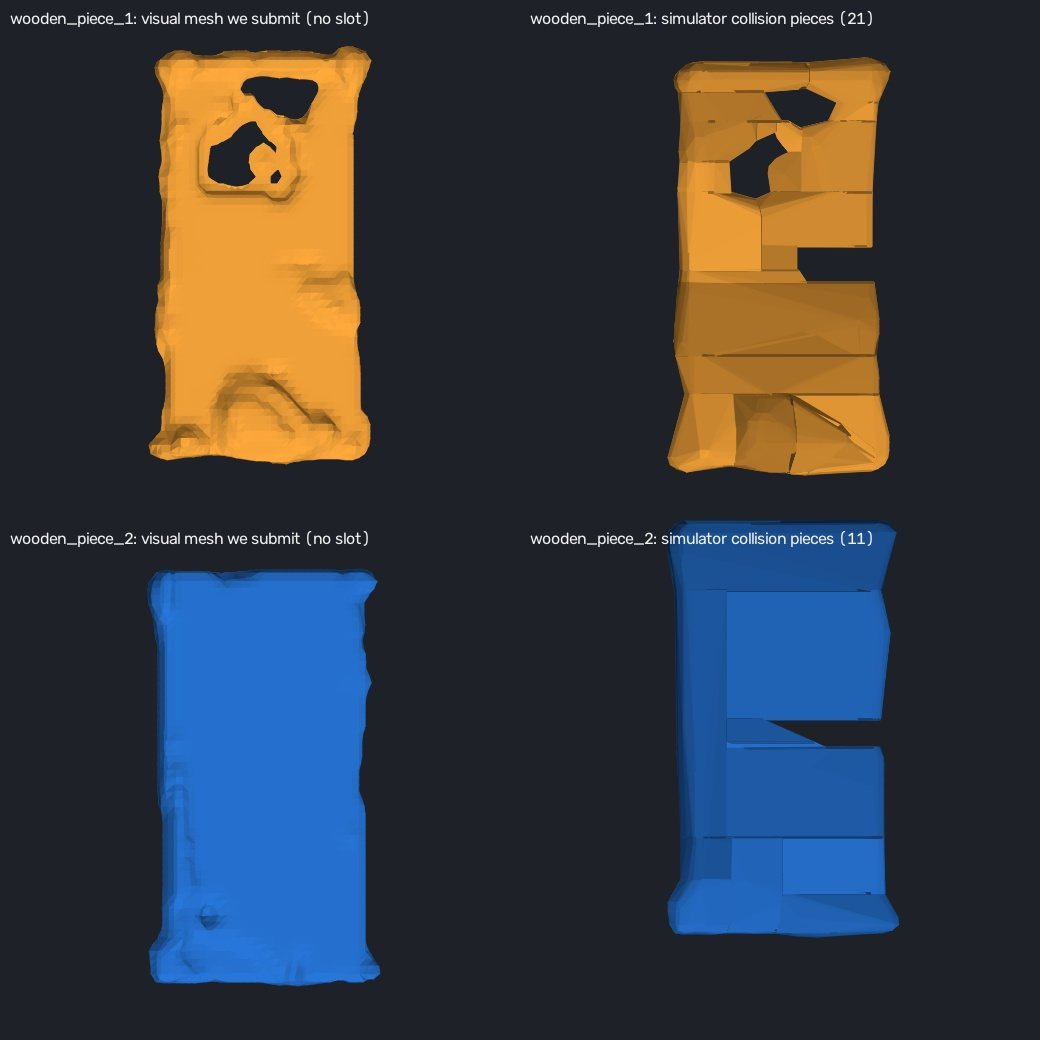
\includegraphics[width=\linewidth]{figures/fig04_boards_collision.jpg}
\caption{Eval 25, the two wooden boards: the visual mesh we submit (no slot) and the carved collision copy the simulator uses (with slot). Only the collision copy lets the boards interlock.}
\label{fig:4}
\end{figure}
\end{itemize}
\subsection{References and grasps}
The reference is what the policy follows: per-frame object poses plus wrist and finger targets retargeted from the perceived hands. Its main steps:

\begin{itemize}[itemsep=2pt,topsep=3pt]
\item \textbf{Table plane.} A robust plane fit under the objects. The first end-to-end score was 0.009 because the fit chose the floor.
\item \textbf{Contact-anchored retargeting.} Fingertips snap to object contacts and the wrist follows. On public ep24, frames with the robot hand inside an object fell from 242 of 275 to 62.
\item \textbf{Support repairs.} For example a curved foot for the pitcher, whose mesh lacked half its base (public ep21: 0.6565 → 0.7723).
\item \textbf{Grasp lock.} A grasp is evolved (64 candidates × 4 jittered copies, 20 generations), locked during the carry, and fine-tuned by 70M steps of RL. On public ep39 it scored 0.958 ± 0.002, against 0.802 ± 0.280 for plain RL.
\item \textbf{Spoon recipe.} A wrap grasp round the handle, a stiffer wrist and an RL fine-tune. Eval 35 scored 0.978 against 0.29–0.34 for RL alone, measured against our own reference. The stiffer wrist is a disclosed embodiment choice.
\end{itemize}
\subsection{Policies}
Each eval episode got its own policy. We trained it with the kit's SAC recipe for 250M steps on 4,096 parallel simulated worlds, at about 45,000 steps per second on one GPU. During training a virtual object controller helps the object along and then fades out, much as in DexMachina \cite{r5}.

Four of our changes mattered. We played references at real speed: the kit's default of half speed caps public AUC at 0.415 even with perfect inputs, below the do-nothing score of 0.446 {[}M{]}. We made an object point-match reward the default. We fixed an inertia bug that made spoon episodes explode early in training. And on 25 October the owner ruled that each episode could use whichever of two learners followed the same reference better over five runs.

The biggest single policy gain came from a silent physics failure. Eval 10, two nested cups, sat at 0.450 ± 0.007 for a week, and four pre-registered fixes failed. On 31 October an agent counted about 6 million overflow warnings per training seed. The contact solver needed up to about 1,050 rows against a limit of 512 and silently dropped the rest. Training at a limit of 1,024, while scoring at the stock limit, lifted eval 10 to about 0.90 on our proxy and the board AUC by +0.020 (pack 11).

\begin{figure}[tbp]
\centering
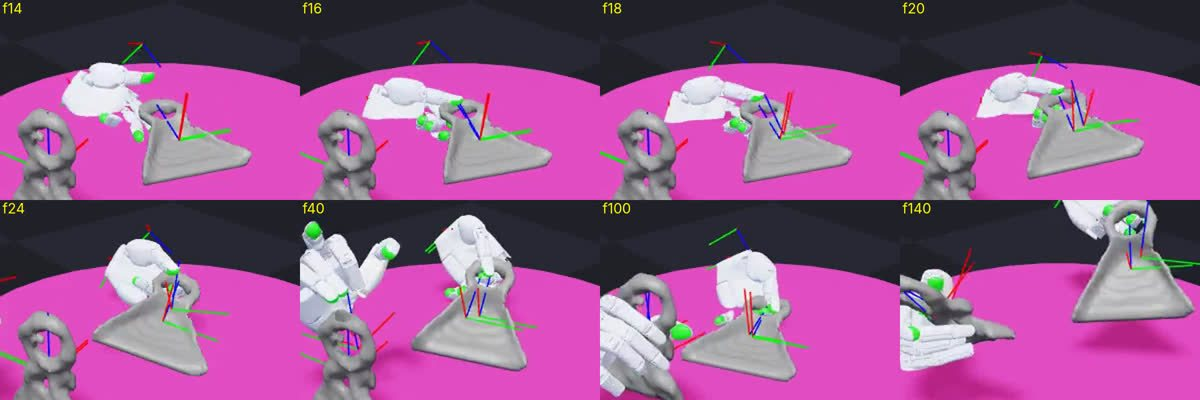
\includegraphics[width=\linewidth]{figures/fig05_robot_dustpan.jpg}
\caption{An RL policy in simulation: the robot hand picks up the dust pan, frame by frame.}
\label{fig:5}
\end{figure}
\subsection{Selection without ground truth}
On eval episodes the only available score is our own. We call it sim\_vs\_ref: the kit's error measure, computed between a rollout and our own reference. On 27 stored public policies it correlated at 0.997 with the true score, and it ranked all 63 pairs correctly that differed by 0.02 or more {[}M{]}. But it cannot see a wrong reference. By 3 November all 20 submitted rollouts passed both success thresholds against our references, while the board counted 2 SP-SR and 4 MP-SR failures.

Single runs were also noisy. On hard episodes, runs of one checkpoint spread with standard deviations of 0.07 to 0.26. So seeds 42 and 43 were fixed in advance, and swaps went through the swap rule and two-host confirmation (section 4.3).

\subsection{Packing and submission}
A pack holds 20 rollouts and the submitted meshes. Packing used an empty folder, a checksum and a byte diff of every file. This came in after an early copy bug shipped four stale rollouts (about -0.005 AUC {[}E{]}). Each upload description names its base pack, its changes, its commit and any disclosed choice. Uploads cost nothing, so a pack aimed at one board went up as a separate variant.

\section{Results}
\subsection{Score trajectory}
\begin{table}[tbp]
\centering\small
\begin{tabularx}{\linewidth}{lllll}
\toprule
\textbf{Board} & \textbf{Pack 1 (24 Oct)} & \textbf{Best} & \textbf{From pack} & \textbf{Change} \\
\midrule
AUC & 0.57468 & 0.88571 & 14p & +0.31103 \\
SP-SR & 0.45 & 0.90 & 12e and later & +0.45 \\
MP-SR & 0.35 & 0.80 & 12e and later & +0.45 \\
RPE (cm) & 12.58 & 2.21 & 14p & -10.37 \\
MPPE (cm) & 8.66 & 1.80 & 14p & -6.86 \\
CD-O (cm) & 0.40513 & 0.23856 & 13j & -0.16657 \\
\bottomrule
\end{tabularx}
\end{table}
The 26 uploads ran from 24 October 18:41 to 3 November 10:30 UTC. The first scored 0.575 and placed 9th on AUC. Pack 3 jumped to 0.789 on 25 October, 4th on AUC that day. A week of small swaps followed (0.811–0.815) while other teams passed us. Then came the eval-10 fix (0.839, 1 November) and the mesh work of 2 November (0.869, then 0.886 the same night).

\begin{figure}[tbp]
\centering
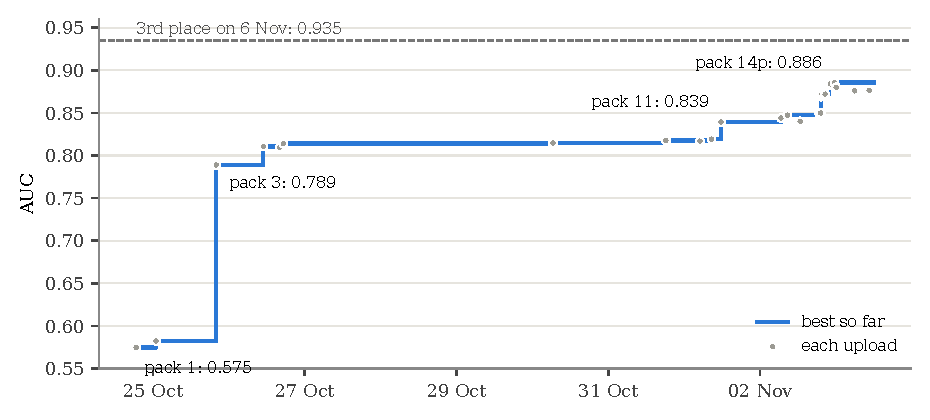
\includegraphics[width=\linewidth]{figures/fig06_auc_by_upload.pdf}
\caption{AUC for each of the 26 uploads, with the best-so-far line. The late dips are planned CD-O variants that gave up AUC to lower CD-O; each board keeps the best upload, so they cost nothing.}
\label{fig:6}
\end{figure}
\subsection{Attribution by lever}
Each kept change was uploaded on top of a known base, so its board effect can be read directly. Grouped by lever:

\begin{table}[tbp]
\centering\small
\begin{tabularx}{\linewidth}{>{\raggedright\arraybackslash}Xlll}
\toprule
\textbf{Lever} & \textbf{AUC change} & \textbf{Share of the gain} & \textbf{Uploads} \\
\midrule
Detection fix and seed picks (pack 2) & +0.00784 & 2.5 \% & 1 \\
Reference rebuild, second learner, identity fixes (pack 3) & +0.20641 & 66.4 \% & 1 \\
Simulator collision carving (pack 4) & +0.02163 & 7.0 \% & 1 \\
Policy retrains and training fixes & +0.02401 & 7.7 \% & 4 \\
Reference repairs and lift windows & +0.00745 & 2.4 \% & 4 \\
Submitted meshes and placement & +0.04369 & 14.0 \% & 10 \\
\textbf{Pack 1 (0.57468) → pack 14p (0.88571)} & \textbf{+0.31103} & \textbf{100 \%} &  \\
\bottomrule
\end{tabularx}
\end{table}
The rows add exactly to the total. The mesh row nets out a CD-O variant (pack 12d, -0.00733) that the mesh path ran through. The repair row removes lift-window gains that would otherwise be counted twice. Pack 3 bundled five kinds of fix in one upload, and the logs do not split it.

\begin{figure}[tbp]
\centering
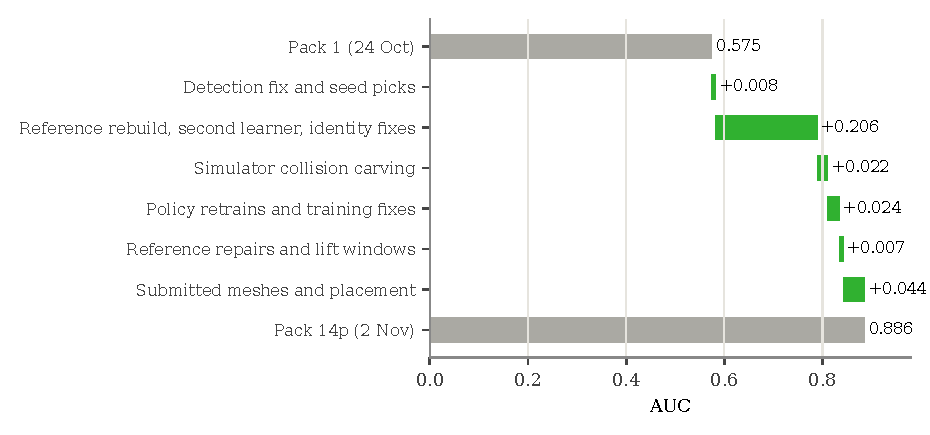
\includegraphics[width=\linewidth]{figures/fig07_auc_bridge.pdf}
\caption{Bridge (waterfall) from pack 1 (0.57468) to pack 14p (0.88571), one bar per lever. One bundle of gross-failure fixes gave two thirds of the gain; submitted meshes were the second lever.}
\label{fig:7}
\end{figure}
Three readings matter:

\begin{enumerate}[itemsep=2pt,topsep=3pt]
\item \textbf{One big fix, then many small ones.} Pack 3 fixed gross failures: objects tracked onto the wrist, swapped board identities, a falling pitcher and failed learners. After it, a typical kept change was worth +0.001 to +0.005.
\item \textbf{Meshes moved the pose boards.} The Tier B mesh change (pack 12e) altered no pose. It gave +0.029 AUC, -0.75 cm RPE and one more episode on each success board. After 31 October, mesh work produced more pose-board points than all policy work.
\item \textbf{Small swaps did not show.} The per-swap board noise is about ±0.008 AUC. Pack 9b had a proxy gain of +0.0018 and moved the board by -0.0008.
\end{enumerate}
CD-O fell in eight mesh steps from 31 October. Every CD-O prediction from the public scans landed within about 0.001 cm of the board; pack 13j was predicted at 0.2384 and scored 0.23856.

\subsection{Leaderboard position}
\begin{table}[tbp]
\centering\small
\begin{tabularx}{\linewidth}{llllll}
\toprule
\textbf{Board} & \textbf{Ours} & \textbf{Rank 3 Nov} & \textbf{Rank 6 Nov} & \textbf{3rd place 6 Nov} & \textbf{Needed to reach 3rd} \\
\midrule
AUC & 0.88571 & 7 & 9 & 0.93486 & +0.049 \\
SP-SR & 0.90 & 11 & 12 & 1.00 & 2 more episodes \\
MP-SR & 0.80 & 7 & 10 & 1.00 & 4 more episodes \\
RPE (cm) & 2.21325 & 8 & 10 & 1.05155 & 52 \% less error \\
MPPE (cm) & 1.79779 & 8 & 10 & 1.16684 & 35 \% less error \\
CD-O (cm) & 0.23856 & 4 & 5 & 0.23213 & 2.7 \% less error \\
\textbf{Rank sum} &  & \textbf{45 (7th)} & \textbf{56 (8th)} &  &  \\
\bottomrule
\end{tabularx}
\end{table}
The rank sum improved from 62 (11th) on 31 October to 45 (7th) on 3 November. It fell to 56 by 6 November without any new upload of ours, because other teams kept improving. On 6 November we were 8th among the teams that appear in all six top-20 lists. Third place on AUC rose from 0.883 on 30 October to 0.935, and the leader's rank sum was 7. CD-O was the only board within reach of 3rd. Pack 13j beat that morning's 3rd-place value by 0.00044 cm, but another team improved the same morning.

\subsection{Where the remaining error sits}
The evidence points to reconstruction bias, mostly while objects are held, and not to policy following {[}I{]}:

\begin{itemize}[itemsep=2pt,topsep=3pt]
\item All 20 final rollouts pass both success thresholds against our own references, none within 20 \% of a threshold. Yet the board counts 2 SP-SR and 4 MP-SR failures. The gap is between our reference and the truth, about 2–3 cm {[}I{]}.
\item On public episodes, 70 \% of the AUC loss is in hand-held frames {[}M{]}.
\item Oracles on public data, using mocap for diagnosis only, value the removal of a constant offset per object at +0.050 and exact frame-0 alignment at +0.040, against +0.032 for perfect poses on still frames {[}M{]}.
\item The bias is specific to each episode for every object except the pitcher, so it cannot be learned per object from public data.
\end{itemize}
\section{What failed, and by how much}
We logged about 96 failed or declined tests. The first failure set the tone. On 24 October the agents projected 0.68 for the first full run, and the board gave 0.575. The eval references were far worse than the public twins they had been checked on.

\begin{figure}[tbp]
\centering
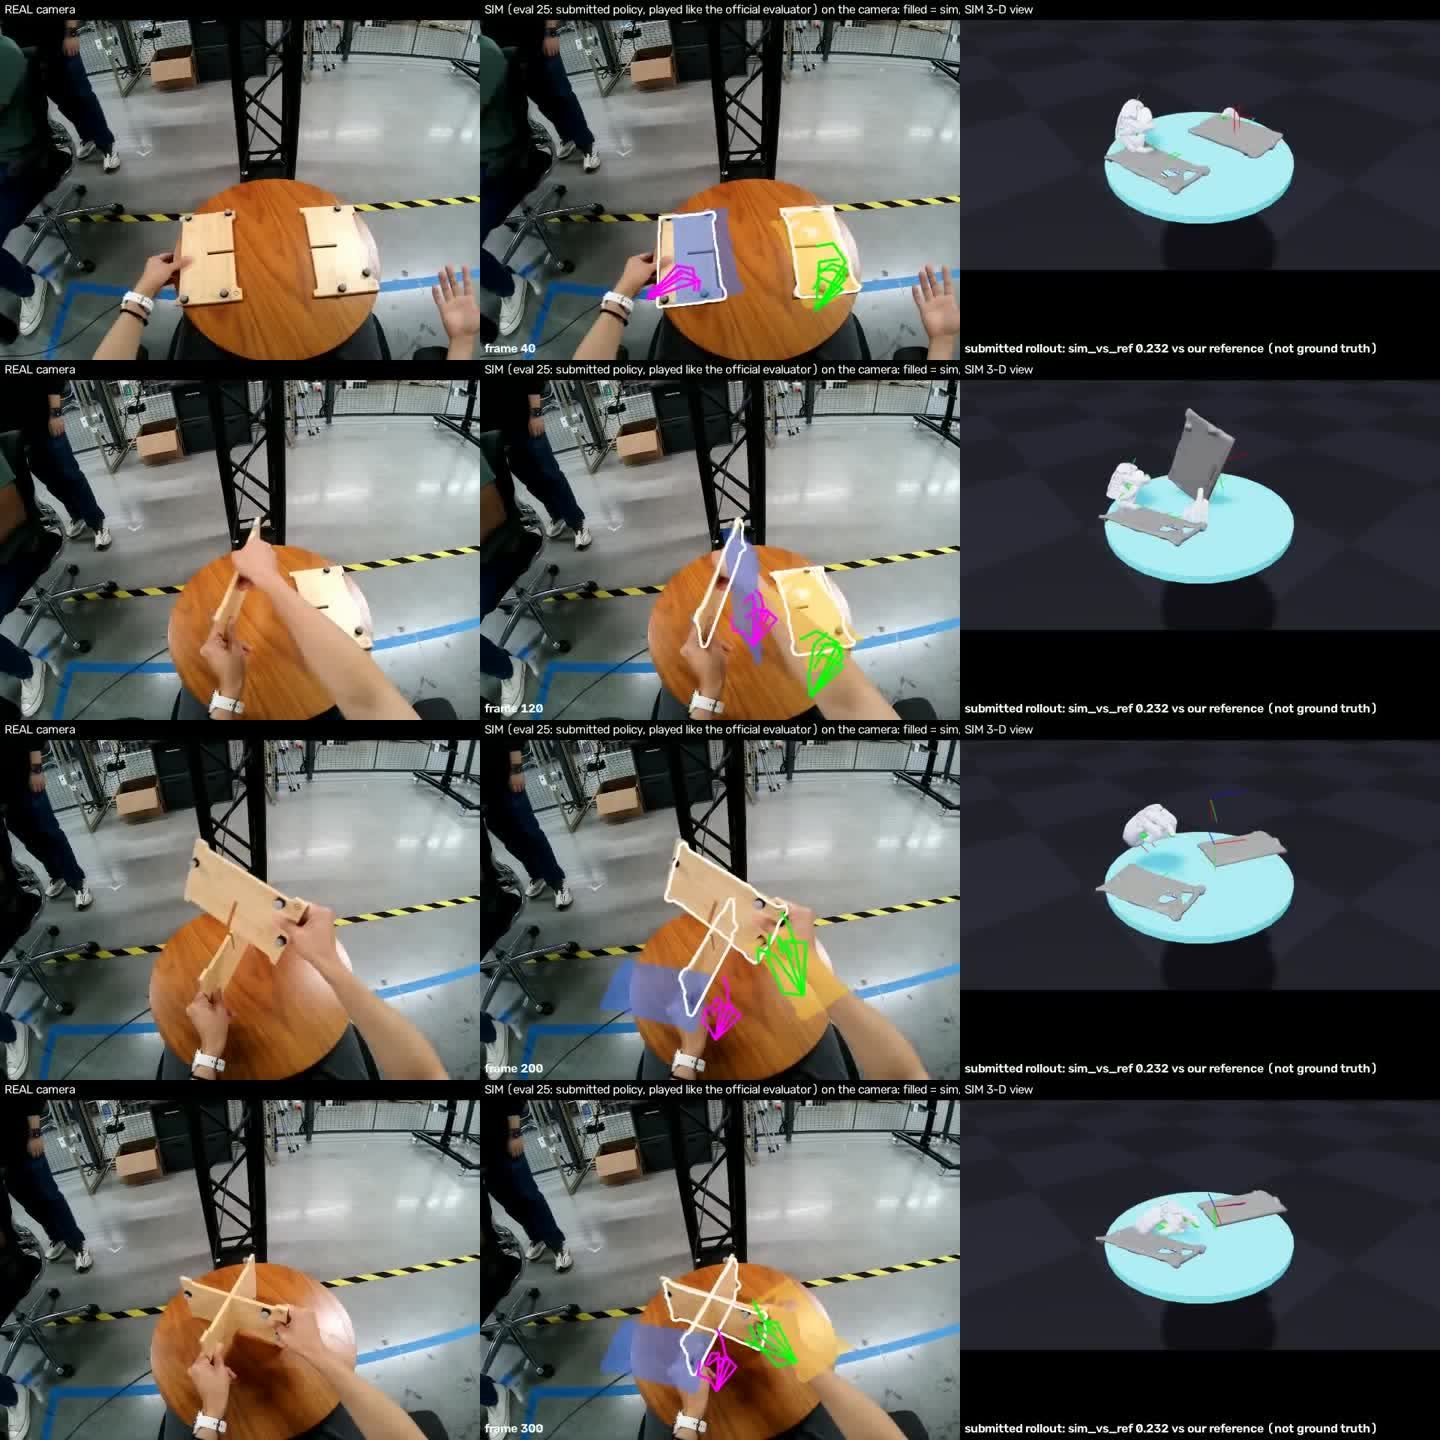
\includegraphics[width=\linewidth]{figures/fig08_first_submission.jpg}
\caption{The first submission's eval-25 rollout (24 October): video frames with our tracks, beside the simulator. The board assembly fails.}
\label{fig:8}
\end{figure}
The table shows the failed tests that cost the most or taught the most. ``Margin'' is the result minus the pass mark, or the board change minus the expected change.

{\small
\begin{longtable}{>{\raggedright\arraybackslash}p{0.116\dimexpr\linewidth-12\tabcolsep\relax}>{\raggedright\arraybackslash}p{0.241\dimexpr\linewidth-12\tabcolsep\relax}>{\raggedright\arraybackslash}p{0.116\dimexpr\linewidth-12\tabcolsep\relax}>{\raggedright\arraybackslash}p{0.116\dimexpr\linewidth-12\tabcolsep\relax}>{\raggedright\arraybackslash}p{0.116\dimexpr\linewidth-12\tabcolsep\relax}>{\raggedright\arraybackslash}p{0.294\dimexpr\linewidth-12\tabcolsep\relax}}
\toprule
\textbf{Date} & \textbf{Test} & \textbf{Pass mark} & \textbf{Result} & \textbf{Margin} & \textbf{Why it failed} \\
\midrule
\endhead
\bottomrule
\endfoot
24 Oct & first full run & projected 0.68 & 0.575 & -0.105 & eval references far worse than public twins \\
26 Oct & lathe pitcher mesh (pack 5), +0.098 on its one public twin & board +0.005 & pitcher -0.0045 & -0.0095 & a single-twin win did not transfer \\
30 Oct & our own human-shaped hand & a gain & -0.161 & -0.161 & perceived fingers 25–40 \% too short \\
31 Oct & realistic object masses & +0.03 on every episode & ep12 -0.013 & -0.043 & mass is a second-order effect \\
31 Oct & per-episode tracking templates & mean +0.01 & -0.170 & -0.18 & template changes break FoundationPose \\
31 Oct & Kalman and RTS \cite{r56} smoothing & +0.005 & RTS -0.00011 & -0.005 & the error is bias plus a half-frame delay \\
31 Oct & correction from mocap-marker blobs & positive & -0.083 & -0.083 & the tracker is already more accurate \\
1 Nov & physics priors (tilt, axis, no floating) & +0.003 & +0.00298 & -0.00002 & the physics cue is no better than the tracker \\
1 Nov & pack 9b policy swap & board gain & -0.0008 & -0.0026 vs proxy & below the board noise \\
2 Nov & cameras from a public room map & bound 0.01 & 0.0029 & -0.007 & camera drift was already 2–9 mm \\
2 Nov & eval-33 reference bridge & +0.02 & +0.0196 & -0.0004 & just below the bar \\
2 Nov & board-2 flip revert (pack 13f1) & board +0.02 & -0.00034 & -0.020 & the hidden scorer likely does not flip it {[}I{]} \\
2–3 Nov & retrains with new collision meshes (6 evals) & swap rule, two hosts & e.g. eval 20 0.604 vs 0.926 & -0.006 to -0.32 & grasps were built on the old shapes \\
3 Nov & learned bias per object & pass per object & 1 of 10 objects & 9 objects fail & the bias is specific to each episode \\
3 Nov & pot pose network & +0.02 & -0.0085 & -0.029 & render-to-real gap, no temporal prior \\
3 Nov & hand-aware ray correction & +0.005 & -0.0042 & -0.009 & depth sees surfaces behind thin boards \\
2–3 Nov & declined: spoon-anchor re-test; eval-35 camera guard & – & not run & – & a probe of the hidden set; a threshold set after seeing scores \\
\end{longtable}
}
Six patterns run through the full catalogue:

\begin{enumerate}[itemsep=2pt,topsep=3pt]
\item \textbf{Most failures were small misses under fixed gates.} The physics priors missed by 0.00002, the eval-33 bridge by 0.0004, an eval-20 collision set by 0.0004. A near-miss counted as a fail. Without written gates, several would have been reported as wins.
\item \textbf{Bias, not noise.} Every smoothing, filtering or second-sensor idea failed. The remaining error was a constant offset, a tilt or a template error, and these methods cannot see it.
\item \textbf{The tracker is fragile to its inputs.} Changes to the template, depth, masks or iterations each broke whole tracks somewhere.
\item \textbf{Policies are tied to the shapes they were trained on.} Better collision meshes broke 6 of 7 retrains.
\item \textbf{Single-twin and single-seed wins do not transfer.} The lathe pitcher, two-hand references and lift windows each rested on one twin or one failed control seed.
\item \textbf{The scorer was read late.} The two biggest late levers came from reading rules and code, not from experiments: the rank sum (31 October) and mesh registration (2 November). The mesh sensitivity had already been measured on 21 October.
\begin{figure}[tbp]
\centering
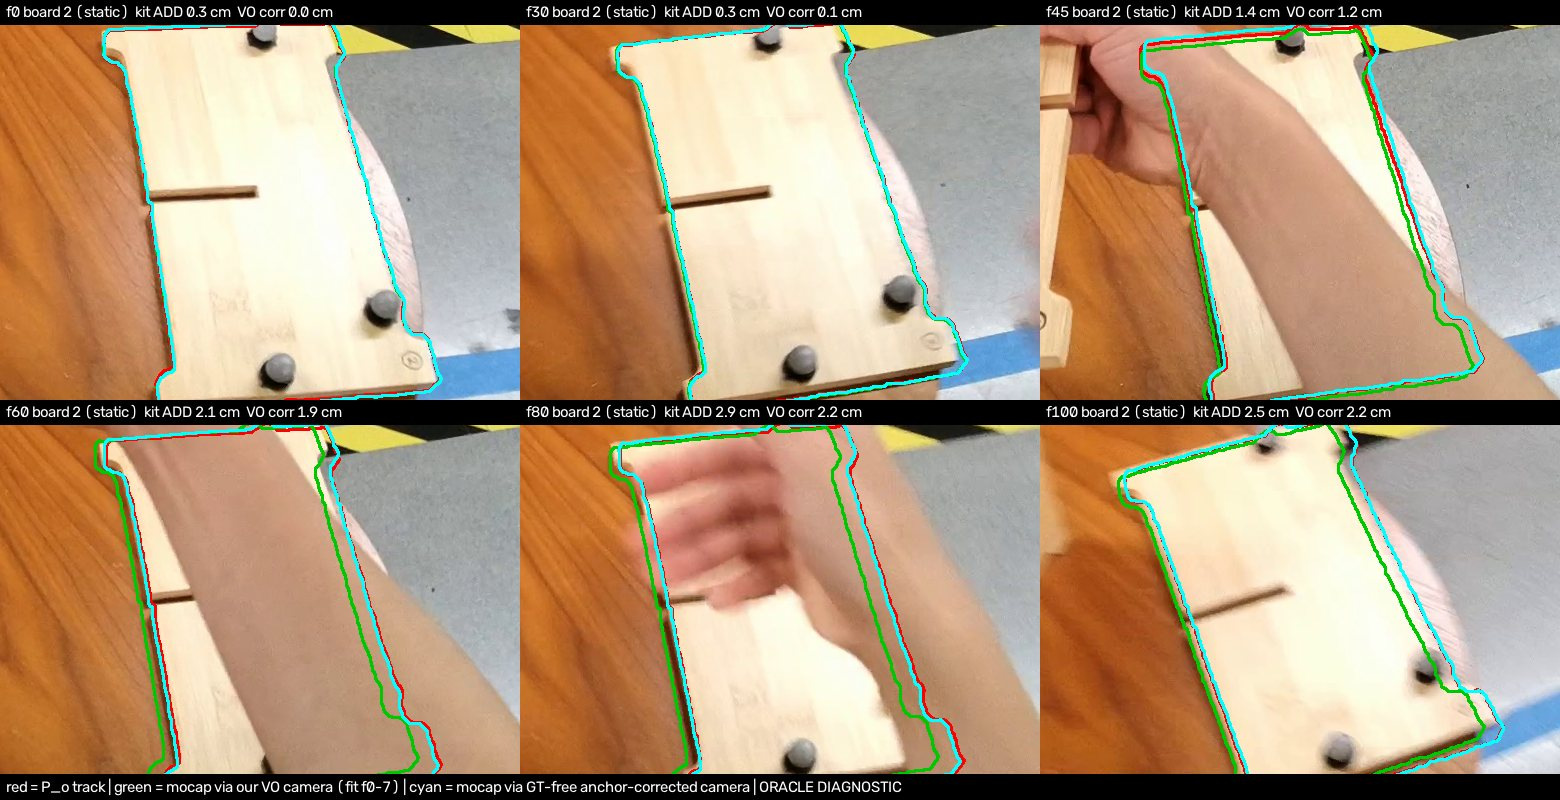
\includegraphics[width=\linewidth]{figures/fig09_heldphase_bias.jpg}
\caption{Public episode 24, board 2 while held: the tracker's outline against the mocap outline. A centimetre-level bias remained after every fix; the mocap is drawn for diagnosis only.}
\label{fig:9}
\end{figure}
\end{enumerate}
\section{Process analysis}
\subsection{Activity}
The record holds 2,359 unique commits on 20 branches: 2,351 by agents and 8 by the owner. While one or two sessions worked (20–25 October), commits ran at 56–104 a day. They fell to 0–41 a day from 26 to 29 October, partly because usage limits paused sessions {[}I{]}. They jumped to 708 on 31 October, the first full day of the lane team. The four lane days, 31 October to 3 November, hold 68 \% of all commits. Uploads came later: 12 of the 26 were on 2 November.

\begin{figure}[tbp]
\centering
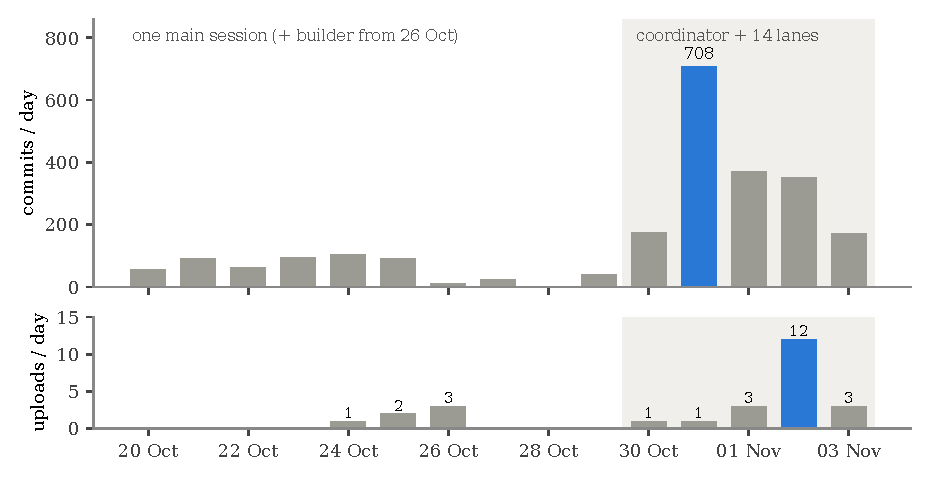
\includegraphics[width=\linewidth]{figures/fig10_activity.pdf}
\caption{Commits per day (bars) and Kaggle uploads per day, 20 October – 3 November. Activity jumped when the lane team started on 31 October; uploads peaked on 2 November, the day meshes became a pose lever.}
\label{fig:10}
\end{figure}
\begin{table}[tbp]
\centering\small
\begin{tabularx}{\linewidth}{ll}
\toprule
\textbf{Measure} & \textbf{Value {[}M{]}} \\
\midrule
Sessions & about 20 \\
Work-log entries & 362 \\
Pre-registration files & 65 \\
Failed or declined tests catalogued & about 96 \\
Kaggle uploads & 26 \\
GPU machines, 20–30 October & 135 machines, 246 GPU-hours \\
\bottomrule
\end{tabularx}
\end{table}
\subsection{How often tests passed}
\begin{itemize}[itemsep=2pt,topsep=3pt]
\item \textbf{Uploads.} 18 of the 25 uploads after the first raised the best AUC. Of the other seven, four were planned CD-O variants and three were failures (packs 5, 9b and 13f1).
\item \textbf{Perception.} Of about 30 ideas tested under gates, three passed: mesh choice, mesh placement, and a half-frame time shift that was never wired into the eval pipeline. All of the roughly 20 GT-free perception ideas tested from 30 October to 3 November failed.
\item \textbf{Policies.} No recipe screen changed the recipe. Retrains with new collision meshes passed 1 time in 7. Lift-window retrains passed 1 time in 8 on their merits, plus once by owner waiver.
\item \textbf{Meshes.} Mesh rounds were the most productive kind of experiment {[}I{]}: three of the four GPU mesh-generation rounds yielded an adopted mesh.
\end{itemize}
\subsection{Cost}
\begin{table}[tbp]
\centering\small
\begin{tabularx}{\linewidth}{>{\raggedright\arraybackslash}Xl}
\toprule
\textbf{GPU item} & \textbf{Amount} \\
\midrule
Estimate before the campaign (18 Oct) & \$110 (\$80–155) {[}E{]} \\
Vast billing, 20–30 Oct & \$376.41 {[}M{]} \\
31 Oct – 3 Nov, from ledgers and credit changes & about \$180 {[}E{]} \\
Campaign total & about \$556 {[}E{]} \\
\bottomrule
\end{tabularx}
\end{table}
Spending was about five times the first estimate. On average the campaign spent about \$18 of GPU per 0.01 AUC gained {[}E{]}. But cost and gain were very uneven:

\begin{table}[tbp]
\centering\small
\begin{tabularx}{\linewidth}{>{\raggedright\arraybackslash}Xll}
\toprule
\textbf{Lever} & \textbf{GPU cost} & \textbf{Board effect} \\
\midrule
Pack 3 batch (13 machines) & \$54.6 {[}M{]} & +0.206 AUC \\
Eval-10 contact-limit diagnostic & \$2.06 {[}M{]} & led to +0.020 AUC \\
Tier B and cross-validated meshes & \$0 (CPU) & +0.040 AUC \\
Three mesh-generation rounds for CD-O & \$21.73 {[}M{]} & with earlier CPU steps, CD-O rank 18th → 4th \\
About 30 perception tests & about \$45 {[}E{]} & one small kept gain (+0.00146) \\
Seven retrains with new collision meshes & about \$47 for the six that failed {[}E{]} & one pass (+0.00168) \\
Recipe screen, 31 Oct & about \$30 {[}E{]} & nothing adopted \\
\bottomrule
\end{tabularx}
\end{table}
Losses to bugs and stalls were small: a few dollars each, such as about \$6.50 on the night of 2–3 November for retrain machines that started without a needed folder. The watchdog destroyed at least one stalled machine (about \$0.90).

AI usage at list price. Every Claude Code session records a running list-price cost after each turn. This is not a bill. The actual AI cost was a \$200 Claude Code subscription plus \$250 of cloud credit gifted by Anthropic {[}M, owner{]}. The list-price figure measures how much work the agents did, not what was paid, and it does not map exactly onto usage limits. Summed over all 20 sessions from their first turn, AI usage came to about \$7,108 {[}M, list price{]}. About \$6,962 of it was competition work (20 October – 3 November). About \$146 was the later writing of the journey report and of this article in the coordinator session (3 November 12:11 to 6 November 16:20 UTC, still growing as this is written). At list price, competition AI usage was about 12 times the GPU spend (about \$556 {[}E{]}); in cash it was below the GPU spend.

Two details of the method matter. A restarted session sometimes resumed its running total from an earlier saved value, so we added only the increases between turns; adding the peaks would have double-counted about \$1,000. For 8 of the 14 lane sessions we read only their later turns; their totals already include the earlier turns unless a restart happened there, so they are lower bounds.

\begin{figure}[tbp]
\centering
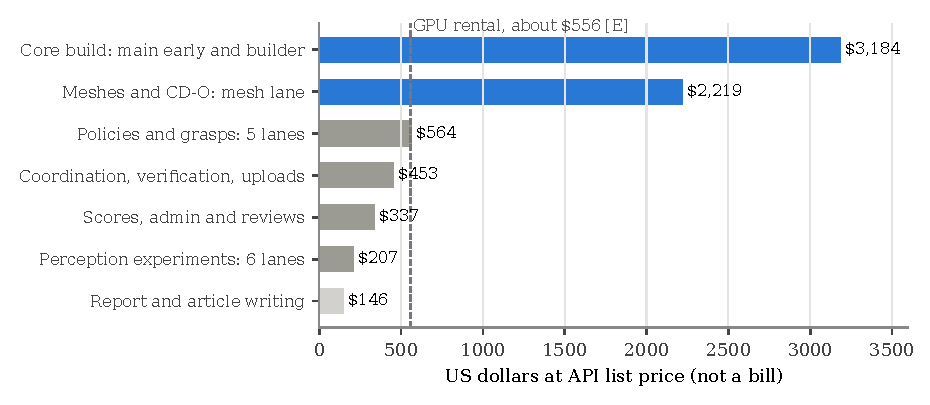
\includegraphics[width=\linewidth]{figures/fig11_ai_usage.pdf}
\caption{AI cost at list price by workstream. Two long-lived build sessions and the mesh lane did about three quarters of the usage; the six perception lanes, which ran most of the pre-registered tests, cost \$207 together. The dashed line is the GPU rental for comparison.}
\label{fig:11}
\end{figure}
What drove the cost was context, not the number of experiments. In the coordinator session's own turns, 98 \% of the tokens processed were cached context being re-read on each turn, and only 0.2 \% were written output: about 620 million re-read tokens against 1.2 million written tokens up to 3 November {[}M{]}. Long-lived sessions with large contexts were expensive (the mesh lane averaged about \$10 a turn), while short single-purpose lanes with a written brief were cheap. The report-writing phase shows the other side: its bulk reading ran on a smaller, cheaper model, which processed about four fifths of that phase's tokens for about 40 \% of its cost {[}M{]}.

\subsection{Human involvement}
The owner sent about 117 messages to the coordinator in five days: 2 on 30 October, 25 on 31 October, 32 on 1 November, 37 on 2 November and 21 on 3 November. That is about 29 a day on the four lane days. Every rule exception, every spending decision and, until the evening of 2 November, every upload passed through him. Usage limits also needed him. One review session hit a limit and sat idle for about 8.8 hours until the owner typed ``Continue''.

\subsection{Agent errors and how each was caught}
\begin{table}[tbp]
\centering\small
\begin{tabularx}{\linewidth}{l>{\raggedright\arraybackslash}X>{\raggedright\arraybackslash}X}
\toprule
\textbf{Error type} & \textbf{Examples} & \textbf{Caught by} \\
\midrule
Over-claimed status & a fix reported as pushed that was not; ``I've emailed'' for a draft; a retrain reported as running that had stopped; an interim ``big win'' & re-checks by the agent itself, the owner, other sessions \\
Numeric artefacts & a search score of 0.584 from simulator state that survived a reset; a checkpoint nearly chosen from stale scores; a score of 0.009 from a floor fit & replays; sanity checks against a do-nothing floor; verifier agents \\
Wrong diagnoses & object overlaps blamed on tracked poses (they were mesh shape); a board swap called a tracking loss; cup spin counted although the board ignores it & follow-up measurement; reading the official code \\
Over-optimistic estimates & 0.74–0.77 projected early, 0.575 scored; a plan priced at \$400–900 that needed \$40–70 & the board; the owner's questions \\
Pipeline bugs that cost money & stale rollouts packed by a copy that would not overwrite; inputs kept off a GPU machine by an ignore rule; missing folders on retrain machines & checksums, failed jobs, the watchdog \\
Integrity leaks & marker radii and wall thickness traced to public scans; early mesh libraries templated on scans; scan copies inside scoring folders & reviews and provenance audits, not gates \\
Coordination failures & duplicate launches from one go-ahead; crossed messages on a cancelled test; two sessions on one episode; clocks up to an hour off & the owner; the shared ledger; a single uploader \\
\bottomrule
\end{tabularx}
\end{table}
Most errors were small and were corrected in the same chat. The serious ones were integrity leaks, because no automatic gate could see them. After them, every mesh build needed a provenance list for each constant.

\subsection{What governance did}
What worked:

\begin{itemize}[itemsep=2pt,topsep=3pt]
\item \textbf{Pre-registration} rejected near-misses that would otherwise have been adopted, and blocked choices made after seeing scores (a room-map guard, a tracking variant picked after scoring).
\item \textbf{No cherry-picking.} The packed runs were already lucky: ten fresh runs of the pack-6 checkpoints averaged 0.8755, against 0.9164 packed (z about 3.2). Packing the best of several runs would have added luck that a reproduction could not repeat {[}I{]}.
\item \textbf{The swap bar and two-host checks} stopped swaps that would have been coin flips on the board.
\item \textbf{Self-destroying machines, the watchdog and the ledger} kept losses to stalls and bugs at a few dollars each.
\item \textbf{The product's safety check} kept the owner in the loop on uploads until he lifted that requirement himself.
\end{itemize}
What worked less well:

\begin{itemize}[itemsep=2pt,topsep=3pt]
\item Integrity leaks were found by review, not by gates.
\item Rules were bent with approval: the eval-15 waiver, the \$6 cap and a standing GPU go-ahead that conflicted with the plan-first rule. The lane in question kept stating plans anyway.
\item Two lane records disagree on whether the owner said yes or no to one test, and the sources do not reconcile them.
\item No rule said ``read the scorer and the ranking rule first''. We think that gap cost more than any single failed test {[}I{]}.
\end{itemize}
\section{Lessons}
\subsection{For learning robot policies from human video}
\begin{enumerate}[itemsep=2pt,topsep=3pt]
\item \textbf{Read the scorer and the ranking rule first.} Mesh registration and the rank sum were worth more late points than any experiment, and both were in the code and the FAQ well before we used them.
\item \textbf{Fix gross failures first.} Objects tracked onto a wrist, swapped look-alikes and falling objects cost far more than centimetre precision. One pack that fixed them gave two thirds of our points.
\item \textbf{Tell bias from noise before choosing a fix.} Smoothing and second sensors cannot remove a constant offset, a tilt or a template error.
\item \textbf{A mesh has three jobs.} The scored mesh, the tracking template and the collision copy want different shapes. Choose each for its own job.
\item \textbf{Look for silent physics failures.} A contact buffer that overflowed in training, with no error raised, held one episode at its floor for a week.
\item \textbf{A ground-truth-free proxy ranks policies but cannot see a wrong reference.} Pair it with direct audits of the reference.
\item \textbf{Policies are tied to their training shapes.} A new collision geometry needs a rebuilt grasp, not only a retrain.
\item \textbf{Cross-validate over episodes and seeds.} Wins on one twin or one seed did not transfer.
\end{enumerate}
\subsection{For agent-run research}
\begin{enumerate}[itemsep=2pt,topsep=3pt]
\item \textbf{Pre-registration in git works with agents.} It is cheap and auditable, and it rejected near-misses that an eager agent, or a tired human, would likely have kept.
\item \textbf{The human principal is busy.} He sent about 29 messages a day to one session in the busiest phase, and every exception went through him. Plan for that load.
\item \textbf{Give each irreversible channel one owner.} One uploader and one spend ledger ended duplicate launches and crossed uploads.
\item \textbf{Treat agent summaries as claims.} Status reports overstated results several times. Verifier agents and re-measurement caught them.
\item \textbf{Integrity needs provenance, not only guards.} Our guard blocked ground-truth inputs, but scan-derived constants slipped in through code and were found only by review.
\item \textbf{Budget for usage limits and lost context.} Limits stopped sessions for hours, and one lane for about two days. Context limits forced summaries that lost detail.
\item \textbf{Model usage dominates at list price.} At list price, AI usage was about 12 times the GPU rental (\$6,962 against about \$556), but in cash it was a \$200 subscription plus \$250 of gifted credit. Report the list-price usage, the cash cost and the usage limits.
\item \textbf{Parallel lanes produce negative results fast.} The lanes produced much of the catalogue in section 7 in four days. That knowledge is useful, but most lanes did not move the board.
\end{enumerate}
\textbf{Budget for context, not for experiments.} Under a flat subscription the limit that binds is the usage cap, not dollars: the cap stopped the first attempt at the journey report. Most usage went to long sessions re-reading their own growing context (section 8.3). The cheapest useful work came from short, single-purpose sessions with a written brief and a pre-registered pass mark: six perception lanes ran their tests for \$207 in total. Bulk reading of logs and transcripts can go to a smaller model, with a stronger model only for the final synthesis.

\section{Limitations and threats to validity}
\begin{itemize}[itemsep=2pt,topsep=3pt]
\item \textbf{n = 1.} One project, one challenge, one owner. There is no human-only team, no single-agent team and no rerun of the official baseline to compare with.
\item \textbf{Mid-table result.} We placed 7th and then 8th, not in the top 3. Lessons from a mid-table entry may not hold for the winning approaches.
\item \textbf{Human-led, not autonomous.} The owner set direction, approved money and made every exception, and advisors shaped key choices. This is a study of a human directing an agent team.
\item \textbf{GT-informed choices.} Some submitted meshes were chosen with public scans, and one revert was informed by a board result. These were disclosed and approved, but they make part of the score less clean than a strict reading of the rules would want.
\item \textbf{Agent-written narrative.} The source report, its digests and this article were written by agents, so self-report bias is possible. Digests were made from turn summaries, not every message, and some disagree. We used the Kaggle record first, then the later and more specific measurement.
\item \textbf{Costs partly estimated.} GPU spend is billed only to 30 October; the total of about \$556 is an estimate. AI usage figures are list-price equivalents from session records; the actual cost was a \$200 subscription plus \$250 of gifted credit. For 8 lane sessions only later turns were read, so their totals are lower bounds.
\item \textbf{Log coverage.} Several sessions were read from turn summaries, so the owner's wording appears only where agents quoted it. One approval time could not be verified, and one lane's GPU spend was not reconciled with the credit balances.
\item \textbf{Literature.} Our reading of several cited works rests on their abstracts. Our search for agent-built entries in embodied-AI competitions was not exhaustive.
\item \textbf{Provisional scores.} Board results stand only once the organisers reproduce the counted files, and the sponsor runs a held-out evaluation after the close.
\end{itemize}
\section{Conclusion}
An agent team directed by one person built a complete pipeline from human video to robot policies. On hidden episodes in a live competition it went from 0.575 to 0.886 AUC, at about \$556 of GPU. Its AI usage, worth about \$6,960 at list price, ran on a \$200 subscription and \$250 of gifted cloud credit. Most of the gain came from fixing gross failures and from understanding the scorer. By the end the robot followed our references well; what remained was bias in how we reconstructed held objects.

The process held up where it was written down. Pre-registered pass marks, a fixed swap bar, two-host checks and one uploader stopped many attractive near-misses and kept losses small. It was weaker where nothing was written: reading the scorer early, tracing the origin of every constant, and keeping sessions from crossing. The human principal stayed essential and busy. We think this is the realistic shape of agent-run research today: fast, broad and honest when the rules are explicit, and still dependent on a person to set direction and to say no.

\section*{Statement on AI assistance}
The engineering work, analyses and first draft of this paper were produced by a team of Claude Code agents (Anthropic) directed by the author, as the paper describes. The author is responsible for the content.

\begin{thebibliography}{99}
\bibitem{r1} Qin, Wu, Liu et al. DexMV: Imitation Learning for Dexterous Manipulation from Human Videos. ECCV, 2022. \href{https://arxiv.org/abs/2108.05877}{arXiv:2108.05877}

\bibitem{r2} Patel, Wang, Radosavovic et al. Learning to Imitate Object Interactions from Internet Videos. arXiv preprint, 2022. \href{https://arxiv.org/abs/2211.13225}{arXiv:2211.13225}

\bibitem{r3} Li, Li, Liu et al. ManipTrans: Efficient Dexterous Bimanual Manipulation Transfer via Residual Learning. CVPR, 2025. \href{https://arxiv.org/abs/2503.21860}{arXiv:2503.21860}

\bibitem{r4} Liu, Adalibieke, Han et al. DexTrack: Towards Generalizable Neural Tracking Control for Dexterous Manipulation from Human References. ICLR, 2025. \href{https://arxiv.org/abs/2502.09614}{arXiv:2502.09614}

\bibitem{r5} Mandi, Hou, Fox et al. DexMachina: Functional Retargeting for Bimanual Dexterous Manipulation. arXiv preprint, 2025. \href{https://arxiv.org/abs/2505.24853}{arXiv:2505.24853}

\bibitem{r6} Pan, Wang, Qi et al. SPIDER: Scalable Physics-Informed Dexterous Retargeting. arXiv preprint, 2025. \href{https://arxiv.org/abs/2511.09484}{arXiv:2511.09484}

\bibitem{r7} NVIDIA V2D Challenge, Track 3 (Kaggle competition page, ``Track 3 - Egocentric - AUC''). Kaggle, 2026. \href{https://www.kaggle.com/competitions/v2d-challenge-track3-auc}{kaggle.com/competitions/v2d-challenge-track3-auc}, accessed 6 Nov 2026.

\bibitem{r8} Anthropic. Claude Code documentation. Online documentation, 2026. \href{https://code.claude.com/docs}{code.claude.com/docs}, accessed 6 Nov 2026.

\bibitem{r9} Lu, Lu, Lange et al. The AI Scientist: Towards Fully Automated Open-Ended Scientific Discovery. arXiv preprint, 2024. \href{https://arxiv.org/abs/2408.06292}{arXiv:2408.06292}

\bibitem{r10} Schmidgall, Su, Wang et al. Agent Laboratory: Using LLM Agents as Research Assistants. arXiv preprint, 2025. \href{https://arxiv.org/abs/2501.04227}{arXiv:2501.04227}

\bibitem{r11} Xiao, Xie, Zhang et al. ENPIRE: Agentic Robot Policy Self-Improvement in the Real World. CoRL, 2026. \href{https://arxiv.org/abs/2606.19980}{arXiv:2606.19980}

\bibitem{r12} Khandelwal, Gupta. Agent-Driven Autonomous Reinforcement Learning Research: Iterative Policy Improvement for Quadruped Locomotion. arXiv preprint, 2026. \href{https://arxiv.org/abs/2603.27416}{arXiv:2603.27416}

\bibitem{r13} Huang, Xu, Ma et al. Reward Hacking Challenges Oversight of Autonomous Research Agents. arXiv preprint, 2026. \href{https://arxiv.org/abs/2609.28614}{arXiv:2609.28614}

\bibitem{r14} Ding, Nannapaneni, Liu et al. Autonomous Research Agents: A Survey of AI Scientists and the Verification Gap. arXiv preprint, 2026. \href{https://arxiv.org/abs/2608.05179}{arXiv:2608.05179}

\bibitem{r15} Xu, Chao, Bian et al. Dexplore: Scalable Neural Control for Dexterous Manipulation from Reference-Scoped Exploration. CoRL, 2025. \href{https://arxiv.org/abs/2509.09671}{arXiv:2509.09671}

\bibitem{r16} Niu, Lv, Zhang et al. EgoAERO: Learning Dexterous Manipulation from a Single Egocentric Video without Object Assets. arXiv preprint, 2026. \href{https://arxiv.org/abs/2606.08057}{arXiv:2606.08057}

\bibitem{r17} Liu, Cheng, Yin et al. EgoEngine: From Egocentric Human Videos to High-Fidelity Dexterous Robot Demonstrations. arXiv preprint, 2026. \href{https://arxiv.org/abs/2606.12604}{arXiv:2606.12604}

\bibitem{r18} Choi, Oh, Lim. Grasp-and-Lift: Executable 3D Hand-Object Interaction Reconstruction via Physics-in-the-Loop Optimization. arXiv preprint, 2026. \href{https://arxiv.org/abs/2601.18121}{arXiv:2601.18121}

\bibitem{r19} Wang, Wang, Tan et al. CRISP: Contact-Guided Real2Sim from Monocular Video with Planar Scene Primitives. ICLR, 2026. \href{https://arxiv.org/abs/2512.14696}{arXiv:2512.14696}

\bibitem{r20} Ma, Liang, Wang et al. Eureka: Human-Level Reward Design via Coding Large Language Models. ICLR, 2024. \href{https://arxiv.org/abs/2310.12931}{arXiv:2310.12931}

\bibitem{r21} Wen, Trepte, Aribido et al. FoundationStereo: Zero-Shot Stereo Matching. CVPR, 2025. \href{https://arxiv.org/abs/2501.09898}{arXiv:2501.09898}

\bibitem{r22} Wen, Yang, Kautz et al. FoundationPose: Unified 6D Pose Estimation and Tracking of Novel Objects. CVPR, 2024. \href{https://arxiv.org/abs/2312.08344}{arXiv:2312.08344}

\bibitem{r23} Ravi, Gabeur, Hu et al. SAM 2: Segment Anything in Images and Videos. ICLR, 2025. \href{https://arxiv.org/abs/2408.00714}{arXiv:2408.00714}

\bibitem{r24} Minderer, Gritsenko, Houlsby. Scaling Open-Vocabulary Object Detection. NeurIPS, 2023. \href{https://arxiv.org/abs/2306.09683}{arXiv:2306.09683}

\bibitem{r25} Oquab, Darcet, Moutakanni et al. DINOv2: Learning Robust Visual Features without Supervision. TMLR, 2024. \href{https://arxiv.org/abs/2304.07193}{arXiv:2304.07193}

\bibitem{r26} Nguyen, Groueix, Ponimatkin et al. CNOS: A Strong Baseline for CAD-based Novel Object Segmentation. ICCV Workshops (R6D), 2023. \href{https://arxiv.org/abs/2307.11067}{arXiv:2307.11067}

\bibitem{r27} Lin, Liu, Lu et al. SAM-6D: Segment Anything Model Meets Zero-Shot 6D Object Pose Estimation. CVPR, 2024. \href{https://arxiv.org/abs/2311.15707}{arXiv:2311.15707}

\bibitem{r28} Zhang, Bazarevsky, Vakunov et al. MediaPipe Hands: On-device Real-time Hand Tracking. CVPR Workshop on Computer Vision for AR/VR, 2020. \href{https://arxiv.org/abs/2006.10214}{arXiv:2006.10214}

\bibitem{r29} Curless, Levoy. A Volumetric Method for Building Complex Models from Range Images. SIGGRAPH, 1996. \href{https://graphics.stanford.edu/papers/volrange/}{graphics.stanford.edu/papers/volrange}

\bibitem{r30} Wen, Tremblay, Blukis et al. BundleSDF: Neural 6-DoF Tracking and 3D Reconstruction of Unknown Objects. CVPR, 2023. \href{https://arxiv.org/abs/2303.14158}{arXiv:2303.14158}

\bibitem{r31} Lee, Wen, Kang et al. Any6D: Model-free 6D Pose Estimation of Novel Objects. CVPR, 2025. \href{https://arxiv.org/abs/2503.18673}{arXiv:2503.18673}

\bibitem{r32} Fan, Parelli, Kadoglou et al. HOLD: Category-agnostic 3D Reconstruction of Interacting Hands and Objects from Video. CVPR, 2024. \href{https://arxiv.org/abs/2311.18448}{arXiv:2311.18448}

\bibitem{r33} Wang, He, Parelli et al. MagicHOI: Leveraging 3D Priors for Accurate Hand-object Reconstruction from Short Monocular Video Clips. ICCV, 2025. \href{https://arxiv.org/abs/2508.05506}{arXiv:2508.05506}

\bibitem{r34} Zhang, Deng, Ma et al. HaWoR: World-Space Hand Motion Reconstruction from Egocentric Videos. CVPR, 2025. \href{https://arxiv.org/abs/2501.02973}{arXiv:2501.02973}

\bibitem{r35} Hampali, Rad, Oberweger et al. HOnnotate: A Method for 3D Annotation of Hand and Object Poses. CVPR, 2020. \href{https://arxiv.org/abs/1907.01481}{arXiv:1907.01481}

\bibitem{r36} Todorov, Erez, Tassa. MuJoCo: A Physics Engine for Model-Based Control. IROS, 2012, pp. 5026–5033. \href{https://doi.org/10.1109/IROS.2012.6386109}{DOI 10.1109/IROS.2012.6386109}

\bibitem{r37} Google DeepMind and NVIDIA. MuJoCo Warp (MJWarp). GitHub software project, 2025. \href{https://github.com/google-deepmind/mujoco_warp}{github.com/google-deepmind/mujoco\textbackslash{}\_warp}

\bibitem{r38} Wei, Liu, Ling et al. Approximate Convex Decomposition for 3D Meshes with Collision-Aware Concavity and Tree Search. ACM TOG (SIGGRAPH journal track), 2022. \href{https://arxiv.org/abs/2205.02961}{arXiv:2205.02961}

\bibitem{r39} Yamada, Lange, Lu et al. The AI Scientist-v2: Workshop-Level Automated Scientific Discovery via Agentic Tree Search. arXiv preprint, 2025. \href{https://arxiv.org/abs/2504.08066}{arXiv:2504.08066}

\bibitem{r40} Yamada, Lange, Lu et al. Towards End-to-End Automation of AI Research. Nature 651, 914–919, 2026. \href{https://arxiv.org/abs/2606.15497}{arXiv:2606.15497}

\bibitem{r41} Gottweis, Weng, Daryin et al. Accelerating scientific discovery with Co-Scientist. Nature, 2026. \href{https://arxiv.org/abs/2502.18864}{arXiv:2502.18864}

\bibitem{r42} Boiko, MacKnight, Kline et al. Autonomous chemical research with large language models. Nature 624, 570–578, 2023. \href{https://doi.org/10.1038/s41586-023-06792-0}{DOI 10.1038/s41586-023-06792-0}

\bibitem{r43} Shen, Yi, Zhao et al. An Empirical Study of Multi-Agent Collaboration for Automated Research. arXiv preprint, 2026. \href{https://arxiv.org/abs/2603.29632}{arXiv:2603.29632}

\bibitem{r44} Trehan, Chopra. Why LLMs Aren't Scientists Yet: Lessons from Four Autonomous Research Attempts. arXiv preprint, 2026. \href{https://arxiv.org/abs/2601.03315}{arXiv:2601.03315}

\bibitem{r45} Chan, Chowdhury, Jaffe et al. MLE-bench: Evaluating Machine Learning Agents on Machine Learning Engineering. ICLR, 2025. \href{https://arxiv.org/abs/2410.07095}{arXiv:2410.07095}

\bibitem{r46} Wijk, Lin, Becker et al. RE-Bench: Evaluating frontier AI R\&D capabilities of language model agents against human experts. arXiv preprint, 2024. \href{https://arxiv.org/abs/2411.15114}{arXiv:2411.15114}

\bibitem{r47} Starace, Jaffe, Sherburn et al. PaperBench: Evaluating AI's Ability to Replicate AI Research. arXiv preprint, 2025. \href{https://arxiv.org/abs/2504.01848}{arXiv:2504.01848}

\bibitem{r48} Lei, Liu, Zhang et al. From Digital to Physical: Digital Agents as Autonomous Coaches for Physical Intelligence. arXiv preprint, 2026. \href{https://arxiv.org/abs/2601.21570}{arXiv:2601.21570}

\bibitem{r49} Atinafu, Cohen. RewardHackingAgents: Benchmarking Evaluation Integrity for LLM ML-Engineering Agents. arXiv preprint, 2026. \href{https://arxiv.org/abs/2603.11337}{arXiv:2603.11337}

\bibitem{r50} Nosek, Ebersole, DeHaven et al. The Preregistration Revolution. PNAS 115(11):2600–2606, 2018. \href{https://doi.org/10.1073/pnas.1708274114}{DOI 10.1073/pnas.1708274114}

\bibitem{r51} Vaccaro. Preregistration for Experiments with AI Agents. ICML (position paper), 2026. \href{https://arxiv.org/abs/2606.11217}{arXiv:2606.11217}

\bibitem{r52} Kassis, T. Introducing Science Superpowers: Scientific Discipline for Your Research Agent. K-Dense blog, 2026 (updated 28 May 2026). \href{https://www.k-dense.ai/blog/introducing-science-superpowers}{k-dense.ai/blog/introducing-science-superpowers}

\bibitem{r53} Besl, McKay. A Method for Registration of 3-D Shapes. IEEE TPAMI 14(2):239–256, 1992. \href{https://doi.org/10.1109/34.121791}{DOI 10.1109/34.121791}

\bibitem{r54} Chetverikov, Svirko, Stepanov et al. The Trimmed Iterative Closest Point Algorithm. ICPR, 2002. \href{https://doi.org/10.1109/ICPR.2002.1047997}{DOI 10.1109/ICPR.2002.1047997}

\bibitem{r55} Vast.ai. Vast.ai GPU marketplace. Website. \href{https://vast.ai}{vast.ai}

\bibitem{r56} Rauch, Tung, Striebel. Maximum Likelihood Estimates of Linear Dynamic Systems. AIAA Journal 3(8):1445–1450, 1965.

\end{thebibliography}
\end{document}
